\documentclass[fleqn]{article}
\usepackage[nodisplayskipstretch]{setspace}
\usepackage{amsmath, nccmath}
\usepackage{amssymb}
\usepackage{enumitem}
\usepackage{etoolbox}
\usepackage{graphicx}
\usepackage{float}
\usepackage{changepage}
\usepackage{environ,capt-of}

\newcommand{\zerodisplayskip}{
	\setlength{\abovedisplayskip}{0pt}%
	\setlength{\belowdisplayskip}{0pt}%
	\setlength{\abovedisplayshortskip}{0pt}%
	\setlength{\belowdisplayshortskip}{0pt}%
	\setlength{\mathindent}{0pt}}

\makeatletter
	\newenvironment{equationCenter}{\@fleqnfalse\begin{equation*}}{\end{equation*}}
\makeatother

\let\oldfigure\figure% Store original figure float environment
\let\endoldfigure\endfigure
\RenewEnviron{figure}[1][H]{% Update figure environment
  %\par\vspace{\intextsep}% Assume in-text placement, so insert appropriate vertical spacing
  \noindent
  % \patchcmd{<cmd>}{<search>}{<replace>}{<success>}{<failure>}
  \patchcmd{\BODY}{\caption}{\captionof{figure}}{}{}% Replace \caption with \captionof{figure} inside \BODY
  % Set "figure"
  \begin{minipage}{\linewidth}
    \BODY
  \end{minipage}
  %\par\vspace{\intextsep}% Assume in-text placement, so insert appropriate vertical spacing
}

\title{Homework 6}
\author{Owen Sowatzke}
\date{October 30, 2023}

\begin{document}
	\offinterlineskip
	\setlength{\lineskip}{12pt}
	\zerodisplayskip
	\maketitle
	
	\begin{enumerate}[nolistsep]
		\item Show that the function that takes $((x_1, x_2),(y_1,y_2)) \in \mathbb{R}^2 \times \mathbb{R}^2$ to \newline $|x_1y_1| + |x_2y_2|$ is not an inner product on $\mathbb{R}^2$.
		
			To be an inner product the function must satisfy the following properties: positivity, definiteness, additivity in first slot, homogeneity in first slot, and conjuage symmetry.
			
			Check whether the function satisfies first slot additivity.
			
			Consider the following function input:
			
			$((x_1, x_2) + (\bar{x}_1, \bar{x}_2),(y_1,y_2)) = ((x_1 + \bar{x}_1, x_2 + \bar{x}_2),(y_1,y_2))$
			
			The output of the function given this input will be
			
			$|(x_1 + \bar{x}_1)y_1| + |(x_2 + \bar{x}_2)y_2| = |x_1y_1 + \bar{x}_1y_1| + |x_2y_2 + \bar{x}_2y_2|$
			
			To satisfy first slot additivity, we need the function output to be
			
			$(|x_1y_1| + |x_2y_2|) + (|\bar{x}_1y_1| + |\bar{x}_2y_2|)$
			
			Note that this result is not necessarily equal to the function output.
			
			Consider the following counter example:
			
			Let $(x_1,x_2) = (1,1)$, $(\bar{x}_1,\bar{x}_1) = (-1,-1)$, and $(y_1,y_2) = (1,1)$.
			
			Then, the function output will be:
			
			$|(1 - 1)1| + |(1 - 1)1| = |(0)1| + |(0)1| = 0 + 0 = 0$
			
			To satisfy first slot additivity, the function output would need to be:
			
			$(|1(1)| + |1(1)|) + (|(-1)1| + |(-1)1|) = (1 + 1) + (1 + 1) = 4$
			
			Because these results are not equivalent, the provided function does not satisfy first slot additivity. $\therefore$ it is not an inner product on $\mathbb{R}^2$.
			
		\item Suppose, $u$, $v$ are nonzero vectors in $\mathbb{R}^2$. Prove that
		
			\begin{equationCenter}
				\langle u,v \rangle = \Vert u \Vert \Vert v \Vert \cos \theta
			\end{equationCenter}
			
			where $\theta$ is the angle between $u$ and $v$ (thinking of $u$ and $v$ as arrows with initial point at the origin).
			
			\textit{Hint:} Draw the triangle formed by $u$, $v$, and $u-v$; then use the law of cosines.
			
			\begin{figure}[H]				
			\centerline{\fbox{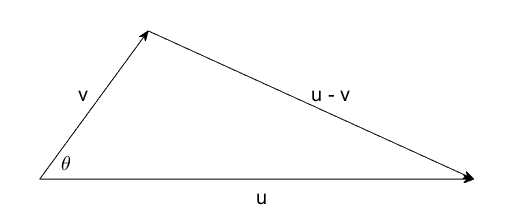
\includegraphics[width=0.5\textwidth]{triangle_prob2.png}}}
			\caption{Triangle Formed by $u$, $v$, and $u - v$}
			\label{triangle_prob2}
			\end{figure}
			
			By the law of cosines:
			
			${\Vert u - v \Vert}^2 = {\Vert u \Vert}^2 + {\Vert v \Vert}^2  - 2{\Vert u \Vert}{\Vert v \Vert}\cos\theta$
			
			Note that ${\Vert u - v \Vert}^2$ can also be expressed as an inner product.
			
			${\Vert u - v \Vert}^2 = \langle u - v, u - v \rangle = \langle u, u - v \rangle + \langle -v, u-v \rangle$
			
			$ = \langle u, u - v \rangle - \langle v, u-v \rangle = (\langle u, u \rangle + \langle u, -v \rangle) - (\langle v, u \rangle + \langle v, -v\rangle)$
			
			$ = (\langle u, u \rangle - \langle u, v \rangle) - (\langle v, u \rangle - \langle v, v\rangle) = \langle u, u \rangle - \langle u, v \rangle - \langle v, u \rangle + \langle v, v\rangle$
			
			$ = \langle u, u \rangle - \langle u, v \rangle - {\langle u, v \rangle}^* + \langle v, v\rangle = \langle u, u \rangle - \langle u, v \rangle - {\langle u, v \rangle} + \langle v, v\rangle$
			
			$ = {\Vert u \Vert}^2 - 2\langle u, v \rangle + {\Vert v \Vert}^2$
			
			Substituting the expression for ${\Vert u - v \Vert}^2$ into the first expression, we get
			
			${\Vert u \Vert}^2 - 2\langle u, v \rangle + {\Vert v \Vert}^2 = {\Vert u \Vert}^2 + {\Vert v \Vert}^2  - 2{\Vert u \Vert}{\Vert v \Vert}\cos\theta$
			
			$\Rightarrow - 2\langle u, v \rangle = - 2{\Vert u \Vert}{\Vert v \Vert}\cos\theta \Rightarrow \langle u, v \rangle = {\Vert u \Vert}{\Vert v \Vert}\cos\theta$
		
		\pagebreak
		\item Suppose $u$, $v \in V$ are such that
		
			\begin{equationCenter}
				\Vert u \Vert = 3 \text{,\quad} \Vert u + v \Vert = 4 \text{,\quad} \Vert u - v \Vert = 6
			\end{equationCenter}
			
			What does $\Vert v \Vert$ equal?
			
			By the parallelogram equality
			
				${\Vert u + v \Vert}^2$ + ${\Vert u - v \Vert}^2 = 2({\Vert u \Vert}^2 + {\Vert v \Vert}^2)$
				
				$\Rightarrow {\Vert u + v \Vert}^2$ + ${\Vert u - v \Vert}^2 = 2{\Vert u \Vert}^2 + 2{\Vert v \Vert}^2$
				
				$\Rightarrow 2{\Vert v \Vert}^2 = {\Vert u + v \Vert}^2$ + ${\Vert u - v \Vert}^2 - 2{\Vert u \Vert}^2$
				
				\begin{equation*}
					\Rightarrow {\Vert v \Vert}^2 = \frac{1}{2}({\Vert u + v \Vert}^2$ + ${\Vert u - v \Vert}^2 - 2{\Vert u \Vert}^2)
				\end{equation*}
				
				\begin{equation*}
					\Rightarrow {\Vert v \Vert} = \sqrt{\frac{1}{2}({\Vert u + v \Vert}^2 + {\Vert u - v \Vert}^2 - 2{\Vert u \Vert}^2)}
				\end{equation*}
				
				\begin{equation*}
					\therefore {\Vert v \Vert} = \sqrt{\frac{1}{2}(4^2 + 6^2 - 2(3^2))} = \sqrt{\frac{1}{2} (16 + 36 - 2(9))}
				\end{equation*}
				
				\begin{equation*}
					 = \sqrt{\frac{1}{2}(52 - 18)} = \sqrt{\frac{1}{2}(34)} = \sqrt{17}
				\end{equation*}
				
			\item Suppose $V$ is a real inner product space. Prove that
			
				\begin{equationCenter}
					\langle u, v\rangle = \frac{{\Vert u + v \Vert}^2 - {\Vert u - v \Vert}^2}{4}
				\end{equationCenter}
				
				for all $u, v \in V$.
				
				${\Vert u + v \Vert}^2 - {\Vert u - v \Vert}^2 = \langle u + v, u + v \rangle - \langle u - v, u - v \rangle$
				
				$ = \langle u, u + v \rangle + \langle v, u + v \rangle - (\langle u, u - v\rangle + \langle -v, u - v \rangle)$
				
				$ = \langle u, u + v \rangle + \langle v, u + v \rangle - (\langle u, u - v\rangle - \langle v, u - v \rangle)$
					
				$ = \langle u, u \rangle + \langle u, v \rangle + \langle v, u \rangle + \langle v, v \rangle - [\langle u, u\rangle + \langle u, -v\rangle - (\langle v, u \rangle + \langle v, -v \rangle)]$
				
				$ = \langle u, u \rangle + \langle u, v \rangle + \langle v, u \rangle + \langle v, v \rangle - [\langle u, u\rangle - \langle u, v\rangle - (\langle v, u \rangle - \langle v, v \rangle)]$
				
				$ = \langle u, u \rangle + \langle u, v \rangle + \langle v, u \rangle + \langle v, v \rangle - (\langle u, u\rangle - \langle u, v\rangle - \langle v, u \rangle + \langle v, v \rangle)$
				
				$ = \langle u, u \rangle + \langle u, v \rangle + \langle v, u \rangle + \langle v, v \rangle - \langle u, u\rangle + \langle u, v\rangle + \langle v, u \rangle - \langle v, v \rangle$
				
				$ = 2\langle u, v \rangle + 2 \langle v, u \rangle = 2(\langle u, v \rangle + \langle v, u \rangle) = 2(\langle u, v \rangle + {\langle u, v \rangle}^*)$
				
				$ = 2(\langle u, v \rangle + \langle u, v \rangle) = 2(2\langle u, v \rangle) = 4\langle u, v \rangle$
				
				Dividing both sides of the equation by 4, we can derive the following result:
				
				\begin{equation*}
					\langle u, v\rangle = \frac{{\Vert u + v \Vert}^2 - {\Vert u - v \Vert}^2}{4}
				\end{equation*}
				
			\item Suppose $V$ is a complex inner product space. Prove that
			
				\begin{equationCenter}
					\langle u, v \rangle = \frac{{\Vert u + v \Vert}^2 - {\Vert u - v \Vert}^2 + {\Vert u + iv \Vert}^2i - {\Vert u - iv \Vert}^2i}{4}
				\end{equationCenter}
				
				for all $u, v \in V$.
				
				${\Vert u + v \Vert}^2 = \langle u + v, u + v \rangle = \langle u, u + v \rangle + \langle v, u + v \rangle$
				
				$ = \langle u, u \rangle + \langle u, v \rangle + \langle v, u \rangle + \langle v, v \rangle$
				
				${\Vert u - v \Vert}^2 = \langle u - v, u - v \rangle = \langle u, u - v \rangle + \langle -v, u - v \rangle$
				
				$ = \langle u, u - v \rangle - \langle v, u - v \rangle = \langle u, u \rangle + \langle u, - v \rangle - (\langle v, u \rangle + \langle v, -v \rangle)$
				
				$ = \langle u, u \rangle - \langle u, v \rangle - (\langle v, u \rangle - \langle v, v \rangle) = \langle u, u \rangle - \langle u, v \rangle - \langle v, u \rangle + \langle v, v \rangle$
				
				${\Vert u + iv \Vert}^2 = \langle u + iv, u + iv \rangle = \langle u, u + iv \rangle + \langle iv, u + iv \rangle$
				
				$ = \langle u, u + iv \rangle + i\langle v, u + iv \rangle = \langle u, u \rangle + \langle u, iv \rangle + i(\langle v, u \rangle + \langle v, iv \rangle)$
				
				$ = \langle u, u \rangle - i\langle u, v \rangle + i(\langle v, u \rangle - i\langle v, v \rangle) = \langle u, u \rangle - i\langle u, v \rangle + i\langle v, u \rangle + \langle v, v \rangle$
				
				${\Vert u - iv \Vert}^2 = \langle u - iv, u - iv \rangle = \langle u, u - iv \rangle + \langle -iv, u - iv \rangle$
				
				$ = \langle u, u - iv \rangle - i\langle v, u - iv \rangle = \langle u, u \rangle + \langle u, -iv \rangle - i(\langle v, u \rangle + \langle v, -iv \rangle)$
				
				$ = \langle u, u \rangle + i\langle u, v \rangle - i(\langle v, u \rangle + i\langle v, v \rangle) = \langle u, u \rangle + i\langle u, v \rangle - i\langle v, u \rangle + \langle v, v \rangle$
				
				$ {\Vert u + v \Vert}^2 - {\Vert u - v \Vert}^2 + {\Vert u + iv \Vert}^2i - {\Vert u - iv \Vert}^2i$
				
				$ = (\langle u, u \rangle + \langle u, v \rangle + \langle v, u \rangle + \langle v, v \rangle)- (\langle u, u \rangle - \langle u, v \rangle - \langle v, u \rangle + \langle v, v \rangle)$
				
				$ + i(\langle u, u \rangle - i\langle u, v \rangle + i\langle v, u \rangle + \langle v, v \rangle) - i(\langle u, u \rangle + i\langle u, v \rangle - i\langle v, u \rangle + \langle v, v \rangle)$
				
				$ = \langle u, u \rangle + \langle u, v \rangle + \langle v, u \rangle + \langle v, v \rangle - \langle u, u \rangle + \langle u, v \rangle + \langle v, u \rangle - \langle v, v \rangle$
				
				$ + i\langle u, u \rangle + \langle u, v \rangle - \langle v, u \rangle + i\langle v, v \rangle - i\langle u, u \rangle + \langle u, v \rangle - \langle v, u \rangle - i\langle v, v \rangle$
				
				$ = 2\langle u, v \rangle + 2\langle v, u \rangle + 2\langle u, v \rangle - 2\langle v, u \rangle = 4\langle u, v \rangle$
				
				\pagebreak
				Dividing both sides of the equation by 4, we can derive the following result:
				
				\begin{equation*}
					\langle u, v \rangle = \frac{{\Vert u + v \Vert}^2 - {\Vert u - v \Vert}^2 + {\Vert u + iv \Vert}^2i - {\Vert u - iv \Vert}^2i}{4}
				\end{equation*}
	\end{enumerate}
\end{document}